%!TEX root = ../Thesis.tex
\chapter{Introduction}
\noindent According to the International Energy Agency \cite{iea}, heat is the largest energy end-use. Providing heating for homes and industrial purposes accounts for around 50\% of the total energy consumption. Renewable heat consumption in the form of bioenergy contribution is expected to grow which will be a better solution for the climate. In relation to the individual consumer, it makes sense to become aware of one's heat consumption, e.g many consumers pay more for their heat consumption than they could. This can be solved by making small adjustments such as replacing radiators with more efficient cooling, replacement of leaky windows, improve insulation of the house etc. Which factors that can influence the heat consumption, are not known to most consumers and thus it can be a challenge to know how to minimize the consumption. \\

\noindent Heat consumption can be described using mathematical models, namely statistical models, and this can lead to an optimization/minimization of the consumption. 
By examining the influence of different physical phenomena, including the temperature, the wind, the sun, etc. on heat consumption, results can be interpreted and visualized for customers.

\section{Introduction to WATTS app}
\begin{wrapfigure}{r}{0.5\textwidth}
    \vspace{-20pt}
      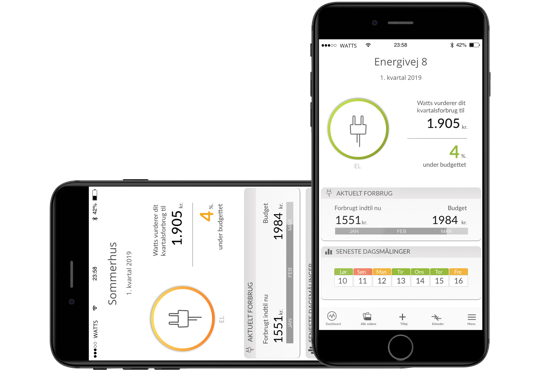
\includegraphics[width=0.48\textwidth]{../../../figures/Watts.png}
    \vspace{-10pt}
  \end{wrapfigure}
The app WATTS is designed and created by the danish energy and optical fibre broadband concern, SEAS-NVE. The app provides several features including an overview of the energy consumption to the consumer by showing the actual consumption and predicting the expected consumption. 
In addition, the app keeps track of the consumers budget and give the user the opportunity to compare their consumption with similar customers. The energy consumption in relation to the expected consumption is visualised with the colours green, yellow and red. The colours are used to indicate whether the consumption is expected to be lower than expected, to exceed the budget by 0-30\%, or to exceed the budget by more than 30\%.
\noindent The app is under expansion such that users are offered the same applications for their heat consumption. In continuation of this, it is possible to add a feature showing the wind dependency on the heat consumption.

\section{Motivation}
The aim of this report is to investigate the tap water consumption and thereby provide possible extensions to the app created by SEAS-NVE, WATTS. By illustrating these features in the app, customers can become aware of their heat consumption and at the same time get a sense of what physical phenomena affect their house. 
\noindent Last but not least, a big part of the motivation is driven by the collaboration with a company. The project thus also has a much more meaningful purpose, namely to develop usable models and make any suggestions on how results can be visualized in an app. \\

\noindent Our approach is to develop statistical models in order to analyse which factors influence the heat consumption. First we will explore the data as daily values and use linear regression models for fitting and predicting with the main focus on the estimates for various significant parameters. Subsequently, we will do a more indepth analysis of data by examining hourly values. The aim is to determine whether the estimates of the different parameters can be improved. 
